\subsection{Glasfaser}
Glasfasern gelten als älteste synthetische Faserart und wurde schon vor 3500 Jahren verwendet. Heute werden Glasfasern aus größtenteils SiO2 und Metalloxiden hergestellt. Die Bestandteile werden bei ca. 1400°C aufgeschmolzen und durch kleine Düsen im Boden des Kessels als dünne Fäden ausgelassen. Die Fäden werden aufgewickelt und zu größeren Fasern verwebt. (Quelle : Konstruieren mit Faserverbund)
Die hohe Festigkeit der Glasfaser beruht auf den kovalenten Bindungen von Silicium (Si) und Sauerstoff (O) Atome. Zugesetzte Metalloxide verhindern eine Ausbildung eines geordneten Gefüges und erhöhen somit zusätzlich die Festigkeit. Die Fasern können in Längsrichtung sehr hohe Kräfte aufnehmen, jedoch nicht in Querrichtung. Dadurch werden sie in eine Matrix eingegossen, die die Querkräfte aufnimmt und die Faser vor dem Knicken schützt. Glasfasern lassen sich auch um enge Radien sehr gut drapieren und sind durch ihre einfache Herstellungsweise sehr preiswert. (Quelle: Handbuch Faserverbund)
Durch die zuvor erläuterten Eigenschaften sind Glasfasern sehr gut für dieses Projekt geeignet, für einen größeren Flügel wäre jedoch der Elastizitätsmodul zu gering und es müsste auf andere Fasern, wie zum Beispiel Kohlefasern zurückgegriffen werden. 
Für die Konstruktion des Flügels stehen die Glasfasern Interglas 90070 und Interglas 92145 des Herstellers Interglas Technologies zur Verfügung. 

\subsection{Matrix}
Um die Fasern vorm Knicken zu schützen wird diese in eine sogenannte Matrix einlaminiert. Diese ist meist ein Polymer wie z.B. Epoxidharz.
\subsection{Netztheorie}
Text folgt noch
\subsection{Klassische Laminatheorie}
Text folgt noch
\subsection{Versagenskriterium nach Puck}
Text folgt noch
\subsection{Bauweise}
In der Aufgabenstellung wird gefordert, dass der Flügel in der Holm-Bauweise konstruiert wird. Ein Holm besteht aus zwei parallelen Gurten, die durch einen oder mehrere Stege miteinander verbunden werden. Dabei bieten sich unterschiedliche Möglichkeiten (s. Abb1). Neben der Festigkeit ist die Steifigkeit die einzige Strukturmechanische Anforderung. Somit lässt sich das Problem als Kragbalken betrachten, der bei der vorgegebenen Prüflast (FPrüf = 100 N) am freien Ende die vorgegebene Durchbiegung (z100N = 22 mm) einhält. Das entstehende Biegemoment wird hauptsächlich von den Gurten getragen, weswegen man sich bei der Wahl des Steges auf andere Kriterien konzentrieren kann. Da keine maximale Torsion vorgegeben ist und die Torsionssteifigkeit fast ausschließlich von der Haut bewirkt wird, führen mehrere Stege, wie man sie bei einem geschlossenen Profil hat, nur zu unerwünschter Gewichtszunahme. Nach diesen Überlegungen haben wir uns für den I-Holm entschieden, da dieser bei einfacher Fertigung die gewünschten Eigenschaften mit sich bringt.
\begin{figure}
	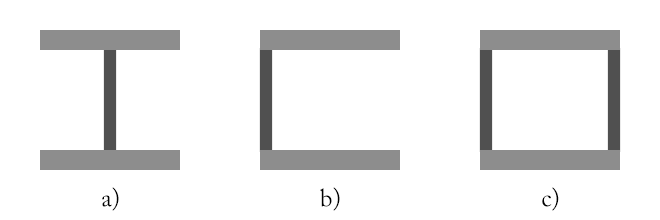
\includegraphics[width=1.0\textwidth]{Bilder/Holmarten.png}
	\caption{a) I-Holm   b) C-Holm    c) Kastenholm}
	\label{fig: Holmarten}
\end{figure} 
Das aerodynamische Profil des Flügels wird durch Schalenbauweise erreicht. Hierbei wir eine dünne Haut nur an kritischen Stellen mit der Sandwichbauweise beziehungsweise Rippen an den kritischen Stellen verstärkt, um Beulen zu verhindern. Die Schale trägt dabei so gut wie gar nicht die Last des Flügels, jedoch ist sie für die Torsionssteifigkeit entscheidend.
